\documentclass[12pt,a4paper]{article}
\usepackage[T1]{fontenc}
\usepackage[utf8]{inputenc}
% es-noshorthands evita un conflicto de babel-spanish con biblatex-apa; es-tabla usa "Tabla"
\usepackage[spanish,es-noshorthands,es-tabla]{babel}
\usepackage{csquotes}
\usepackage{mathptmx}
\usepackage[margin=2.5cm]{geometry}
\usepackage{graphicx}
\usepackage{booktabs}
\usepackage{tabularx}
\usepackage{array}
\usepackage{etoolbox}
\usepackage{float}       % [H]: tablas pequeñas fijas justo donde se mencionan
\usepackage[section]{placeins}  % ninguna tabla o figura cruza al inicio de la sección siguiente
% Permite que tablas y figuras altas compartan página con texto (evita páginas solo de flotantes)
\renewcommand{\topfraction}{0.9}
\renewcommand{\bottomfraction}{0.8}
\renewcommand{\textfraction}{0.07}
\renewcommand{\floatpagefraction}{0.85}
\setcounter{topnumber}{3}
\setcounter{totalnumber}{4}
\setlength{\floatsep}{16pt plus 4pt minus 2pt}       % entre flotantes apilados
\setlength{\textfloatsep}{16pt plus 4pt minus 2pt}   % entre flotante y texto
\usepackage{setspace}
\usepackage{titlesec}
% Leyendas APA 7: "Tabla N" en negrita, título en cursiva en la línea siguiente, ambos arriba
\usepackage[labelfont=bf,textfont=it,labelsep=newline,justification=raggedright,
            singlelinecheck=false,position=top,skip=4pt]{caption}
\usepackage{xurl}
\usepackage[hidelinks]{hyperref}
\usepackage[style=apa,backend=biber]{biblatex}
\addbibresource{refs.bib}
% Lista de referencias alineada a la izquierda (APA); xurl permite cortar URL largas sin estirar espacios
\AtBeginBibliography{\raggedright}

% ── Guía de estilo: Times 12, interlineado 1.5, sangría APA, títulos 12 pt en negrita
\onehalfspacing
\setlength{\parindent}{1.27cm}
\setlength{\parskip}{0pt}
\titleformat{\section}{\normalfont\normalsize\bfseries\centering}{\thesection.}{0.5em}{}
\titleformat{\subsection}{\normalfont\normalsize\bfseries}{\thesubsection.}{0.5em}{}
\titlespacing*{\section}{0pt}{1.2em}{0.6em}
\titlespacing*{\subsection}{0pt}{1em}{0.4em}
% Tablas y figuras: interlineado sencillo; cuerpo de tabla a 11 pt
\AtBeginEnvironment{table}{\singlespacing\small}
\AtBeginEnvironment{figure}{\singlespacing}
\newcolumntype{L}{>{\raggedright\arraybackslash}X}
% Nota APA bajo tablas y figuras
\newcommand{\nota}[1]{\par\smallskip
  \begin{minipage}{\linewidth}\small\raggedright\textit{Nota.}~#1\end{minipage}}
% \input no es expandible dentro de tablas; \@@input (primitiva de TeX) sí
\makeatletter\newcommand{\filas}[1]{\@@input #1 }\makeatother

\begin{document}

% ───────────────────────── Carátula (réplica de Caratula 2023 FISI) ─────────────────────────
\begin{titlepage}
  \singlespacing
  \centering
  {\normalsize “AÑO DE LA ESPERANZA Y EL FORTALECIMIENTO DE LA DEMOCRACIA”}\par
  \vspace{1.6cm}
  {\normalsize UNIVERSIDAD NACIONAL MAYOR DE SAN MARCOS}\par\vspace{0.35cm}
  {\normalsize (Universidad del Perú, Decana de América)}\par\vspace{0.35cm}
  {\normalsize FACULTAD DE INGENIERÍA DE SISTEMAS E INFORMÁTICA}\par\vspace{0.35cm}
  {\normalsize ESCUELA PROFESIONAL DE INGENIERÍA DE SOFTWARE}\par
  \vspace{0.6cm}
  
\includegraphics[width=0.38\textwidth]{figures/escudo_unmsm.png}\par
  \vspace{0.8cm}
  {\normalsize ASIGNATURA:}\par\vspace{0.2cm}
  {\normalsize Software Inteligente}\par\vspace{0.7cm}
  {\normalsize TEMA:}\par\vspace{0.2cm}
  {\normalsize Laboratorio 12: Análisis de AlexNet, entrenamiento desde cero,\\
   extracción de características y \textit{fine-tuning}}\par\vspace{0.7cm}
  {\normalsize DOCENTE:}\par\vspace{0.2cm}
  {\normalsize David Calderón}\par\vspace{0.7cm}
  {\normalsize ESTUDIANTE:}\par\vspace{0.2cm}
  {\normalsize Angela Jara}\par
  \vfill
  {\normalsize 2026}\par\vspace{0.3cm}
  {\normalsize LIMA-PERÚ}\par
\end{titlepage}

% ───────────────────────── 1. Introducción ─────────────────────────
\section{Introducción}

Este informe analiza AlexNet \parencite{krizhevsky2012}, red convolucional preentrenada en ImageNet
\parencite{deng2009}, y resume su uso en tres estrategias de entrenamiento implementadas en el
notebook del laboratorio.\footnote{Notebook: \texttt{laboratorio12\_alexnet\_transfer\_learning.ipynb}.
Se entrega en PDF, en lugar del archivo Word solicitado, por decisión de la estudiante; el contenido
responde a todas las indicaciones del laboratorio.} Se eligió AlexNet porque es una pila simple de
convoluciones, sus conteos de capas no son ambiguos y entrena rápido en CPU. Se usa la implementación de torchvision
\parencite{torchvision_alexnet}, que sigue la variante de \textcite{krizhevsky2014}: 64-192-384-256-256
filtros, sin normalización LRN ni convoluciones agrupadas en dos GPU.

% ───────────────────────── 2. Análisis ─────────────────────────
\section{Análisis de AlexNet}

\subsection{Condiciones de entrada}

AlexNet espera imágenes en color de tamaño fijo, escaladas y normalizadas como en ImageNet
(Tabla~\ref{tab:entrada}).

\begin{table}[H]
\caption{Condiciones de entrada de AlexNet}
\label{tab:entrada}
\begin{tabularx}{\textwidth}{@{}lL@{}}
\toprule
Aspecto & Condición \\
\midrule
Formato & Imagen RGB de 3 canales; tensor de forma $N \times 3 \times H \times W$. \\
Tamaño & $224 \times 224$ nominal; desde unos $63 \times 63$ px gracias al \textit{pooling} adaptativo. \\
Escala & Valores de píxel en $[0, 1]$. \\
Normalización & Media $(0.485, 0.456, 0.406)$ y desviación $(0.229, 0.224, 0.225)$ de ImageNet, por canal. \\
\bottomrule
\end{tabularx}
\end{table}

\subsection{Cantidad de bloques}

AlexNet no define bloques con nombre; aquí se cuenta como bloque cada etapa cerrada por un
\textit{max-pooling}. Resultan \textbf{3 bloques convolucionales} (conv1 \textbar{} conv2 \textbar{}
conv3--conv5) y \textbf{1 bloque clasificador} con 3 capas densas (Tabla~\ref{tab:arq}).

\begin{table}[!tbp]
\caption{Arquitectura de AlexNet (torchvision)}
\label{tab:arq}
\setlength{\tabcolsep}{4.5pt}
\begin{tabular}{@{}lllrlrr@{}}
\toprule
Etapa & Capa & Tipo & \shortstack[r]{Filtros/\\unidades} & \shortstack[l]{Kernel /\\paso / relleno} & Salida & Parámetros \\
\midrule
\filas{generated/arquitectura.tex}
\midrule
\multicolumn{6}{@{}l}{Total} & 61\,100\,840 \\
\bottomrule
\end{tabular}
\nota{Entrada de $224\times224$ y cabeza original de 1000 clases. En las demos, dense3 se reemplaza
por 4096$\to$3 (12\,291 parámetros; total 57\,016\,131). Cada convolución y dense1--dense2 van
seguidas de ReLU; antes de dense1 y dense2 hay \textit{dropout} de 0.5.}
\end{table}

\subsection{Cantidad de convoluciones}

Tiene \textbf{5 capas convolucionales}: conv1 ($11\times11$, 64 filtros, paso 4), conv2 ($5\times5$, 192),
conv3 ($3\times3$, 384), conv4 ($3\times3$, 256) y conv5 ($3\times3$, 256). Las convoluciones suman solo
2.47 M de los 61.1 M parámetros; el resto está en las capas densas.

\subsection{Funciones de activación}

\begin{itemize}
  \item \textbf{ReLU}, $f(x) = \max(0, x)$, tras cada una de las 5 convoluciones y tras dense1 y dense2
  (7 en total). No se satura como \textit{tanh} y, según el artículo original, entrena varias veces más
  rápido \parencite{krizhevsky2012}.
  \item \textbf{Softmax} en la salida: no es una capa del modelo; la aplica la pérdida de entropía
  cruzada al entrenar y se usa para obtener probabilidades al predecir.
  \item El \textit{dropout} (0.5) es regularización, no activación.
\end{itemize}

\subsection{Funciones de optimización}

El modelo no fija un optimizador: se elige al entrenar. El artículo original usó \textbf{SGD} con
lotes de 128, \textit{momentum} 0.9, \textit{weight decay} $5\times10^{-4}$ y LR inicial 0.01,
dividido entre 10 cuando el error de validación dejaba de mejorar \parencite{krizhevsky2012}. El
notebook usa el mismo SGD (\textit{momentum} 0.9, \textit{weight decay} $5\times10^{-4}$) con un LR
distinto por estrategia (Tabla~\ref{tab:ent}). También pueden usarse Adam o RMSprop, que adaptan el
paso por parámetro.

\begin{table}[H]
\caption{Configuración de entrenamiento por estrategia}
\label{tab:ent}
\begin{tabularx}{\textwidth}{@{}lrrLL@{}}
\toprule
Estrategia & LR & \shortstack[r]{Épocas\\máx.} & Capas entrenables & Motivo \\
\midrule
\filas{generated/entrenamiento.tex}
\bottomrule
\end{tabularx}
\nota{Las tres estrategias usan SGD con \textit{momentum} 0.9, \textit{weight decay} $5\times10^{-4}$,
lotes de 32 y parada temprana con paciencia 5.}
\end{table}

\subsection{Parámetros configurables}

La Tabla~\ref{tab:param} resume los parámetros que se pueden ajustar, del modelo y del
entrenamiento, junto con el objetivo de cada uno y el valor usado en el notebook.

\begin{table}[!tbp]
\caption{Parámetros configurables de AlexNet y de su entrenamiento}
\label{tab:param}
\begin{tabularx}{\textwidth}{@{}lLl@{}}
\toprule
Parámetro & Objetivo & Valor usado \\
\midrule
\multicolumn{3}{@{}l}{\textit{Del modelo} (\texttt{models.alexnet})} \\
\texttt{weights} & Pesos iniciales: \texttt{None} (aleatorios) o preentrenados en ImageNet. & \texttt{None} / \texttt{IMAGENET1K\_V1} \\
\texttt{progress} & Mostrar la barra de descarga de los pesos. & \texttt{True} \\
\texttt{num\_classes} & Número de salidas; solo se puede cambiar sin pesos preentrenados. & 3 (desde cero) \\
\texttt{dropout} & Probabilidad de apagar neuronas del clasificador para reducir sobreajuste. & 0.5 \\
\midrule
\multicolumn{3}{@{}l}{\textit{Por capa}} \\
\texttt{requires\_grad} & Congelar (\texttt{False}) o entrenar (\texttt{True}) los pesos de cada capa. & ver Tabla~\ref{tab:ent} \\
Reemplazo de capa & Adaptar la salida a un problema nuevo. & dense3 $\to$ \texttt{Linear(4096, 3)} \\
\midrule
\multicolumn{3}{@{}l}{\textit{Del entrenamiento}} \\
Optimizador & Regla para actualizar los pesos. & SGD \\
\texttt{lr} & Tamaño del paso de cada actualización. & 0.01 / 0.001 / 0.0001 \\
\texttt{momentum} & Suavizar la dirección del paso usando los anteriores. & 0.9 \\
\texttt{weight\_decay} & Penalizar pesos grandes (regularización L2). & $5\times10^{-4}$ \\
Pérdida & Medir el error de clasificación. & Entropía cruzada \\
\texttt{batch\_size} & Imágenes por actualización. & 32 \\
Épocas máx. & Límite de pasadas por los datos. & 30 / 10 / 10 \\
\texttt{patience} & Épocas sin mejorar la validación antes de detener. & 5 \\
Tamaño de entrada & Resolución de las imágenes. & $224\times224$ \\
Aumento de datos & Variar las imágenes de entrenamiento para generalizar mejor. & recorte, volteo, rotación $\pm15^\circ$ \\
\bottomrule
\end{tabularx}
\nota{Los valores separados por barras corresponden a desde cero / solo capa clasificadora /
\textit{fine-tuning}.}
\end{table}

\subsection{¿Permite agregar capas?}

\textbf{Sí.} El modelo está formado por contenedores \texttt{nn.Sequential} (\texttt{features},
\texttt{classifier}) cuyas capas se pueden reemplazar o a los que se pueden añadir capas nuevas. La
demo 2 reemplaza dense3 por una capa nueva de 3 salidas (notebook §6).

\subsection{¿Permite \textit{fine-tuning}?}

\textbf{Sí.} Cada parámetro tiene el atributo \texttt{requires\_grad}, que permite congelar o
descongelar capas individuales. La demo 3 descongela conv4 y conv5, mantiene congeladas conv1--conv3
y dense1--dense2, y entrena con un LR 10 veces menor (notebook §7).

\subsection{¿Permite hacer entrenamiento específico?}

\textbf{Sí.} Las características aprendidas en ImageNet (bordes, texturas, partes de objetos) se
reutilizan para un problema nuevo con otras clases: aprendizaje por transferencia. Las demos 2 y 3
adaptan AlexNet a diagnosticar enfermedades en hojas de frijol, un dominio que no está entre las
categorías de ImageNet (notebook §6–§7). Otra opción es reentrenar todo el clasificador en lugar de
solo la última capa.

% ───────────────────────── 3. Resultados ─────────────────────────
\section{Implementación y resultados}

Se usó el conjunto \textit{Beans} \parencite{makerere2020beans}: fotografías reales de hojas de frijol
en 3 clases (mancha angular, roya y sana), con su partición oficial de 1034 imágenes de
entrenamiento, 133 de validación y 128 de prueba (licencia MIT). Las tres estrategias comparten
partición, preprocesamiento, aumento de datos y conjunto de prueba (Tabla~\ref{tab:res}). Una
primera ejecución con Rock-Paper-Scissors (imágenes sintéticas) se descartó: allí el modelo desde
cero alcanzó 99.5\,\% y superó a la transferencia (96\,\%), porque el problema era demasiado fácil para
mostrar su beneficio.

\begin{table}[!tbp]
\caption{Comparación de las tres estrategias}
\label{tab:res}
\begin{tabular*}{\textwidth}{@{\extracolsep{\fill}}lrcrcc@{}}
\toprule
Estrategia & \shortstack{Parám.\\entrenables} & \shortstack{Épocas\\(mejor)} & \shortstack{Tiempo\\(min)} & \shortstack{Exactitud\\val.} & \shortstack{Exactitud\\prueba} \\
\midrule
\filas{generated/resultados.tex}
\bottomrule
\end{tabular*}
\nota{Entrenamiento en CPU (10 hilos). La exactitud de validación corresponde a la mejor época; la
de prueba se mide una sola vez al final de cada estrategia.}
\end{table}

Con solo la capa nueva entrenada (12\,291 parámetros), la transferencia logra 85.9\,\% en prueba
frente a 77.3\,\% desde cero, en una quinta parte del tiempo y con 85\,\% de validación desde la
primera época (Figura~\ref{fig:curvas}). El \textit{fine-tuning} de conv4--conv5 obtiene la mejor
validación (92.5\,\%) pero empata en prueba (110 de 128 aciertos); con 128 imágenes cada acierto vale
0.8 puntos. En las tres estrategias el error dominante es confundir mancha angular con roya
(Figura~\ref{fig:matrices}).

\begin{figure}[!tbp]
\caption{Curvas de pérdida y exactitud por estrategia}
\label{fig:curvas}
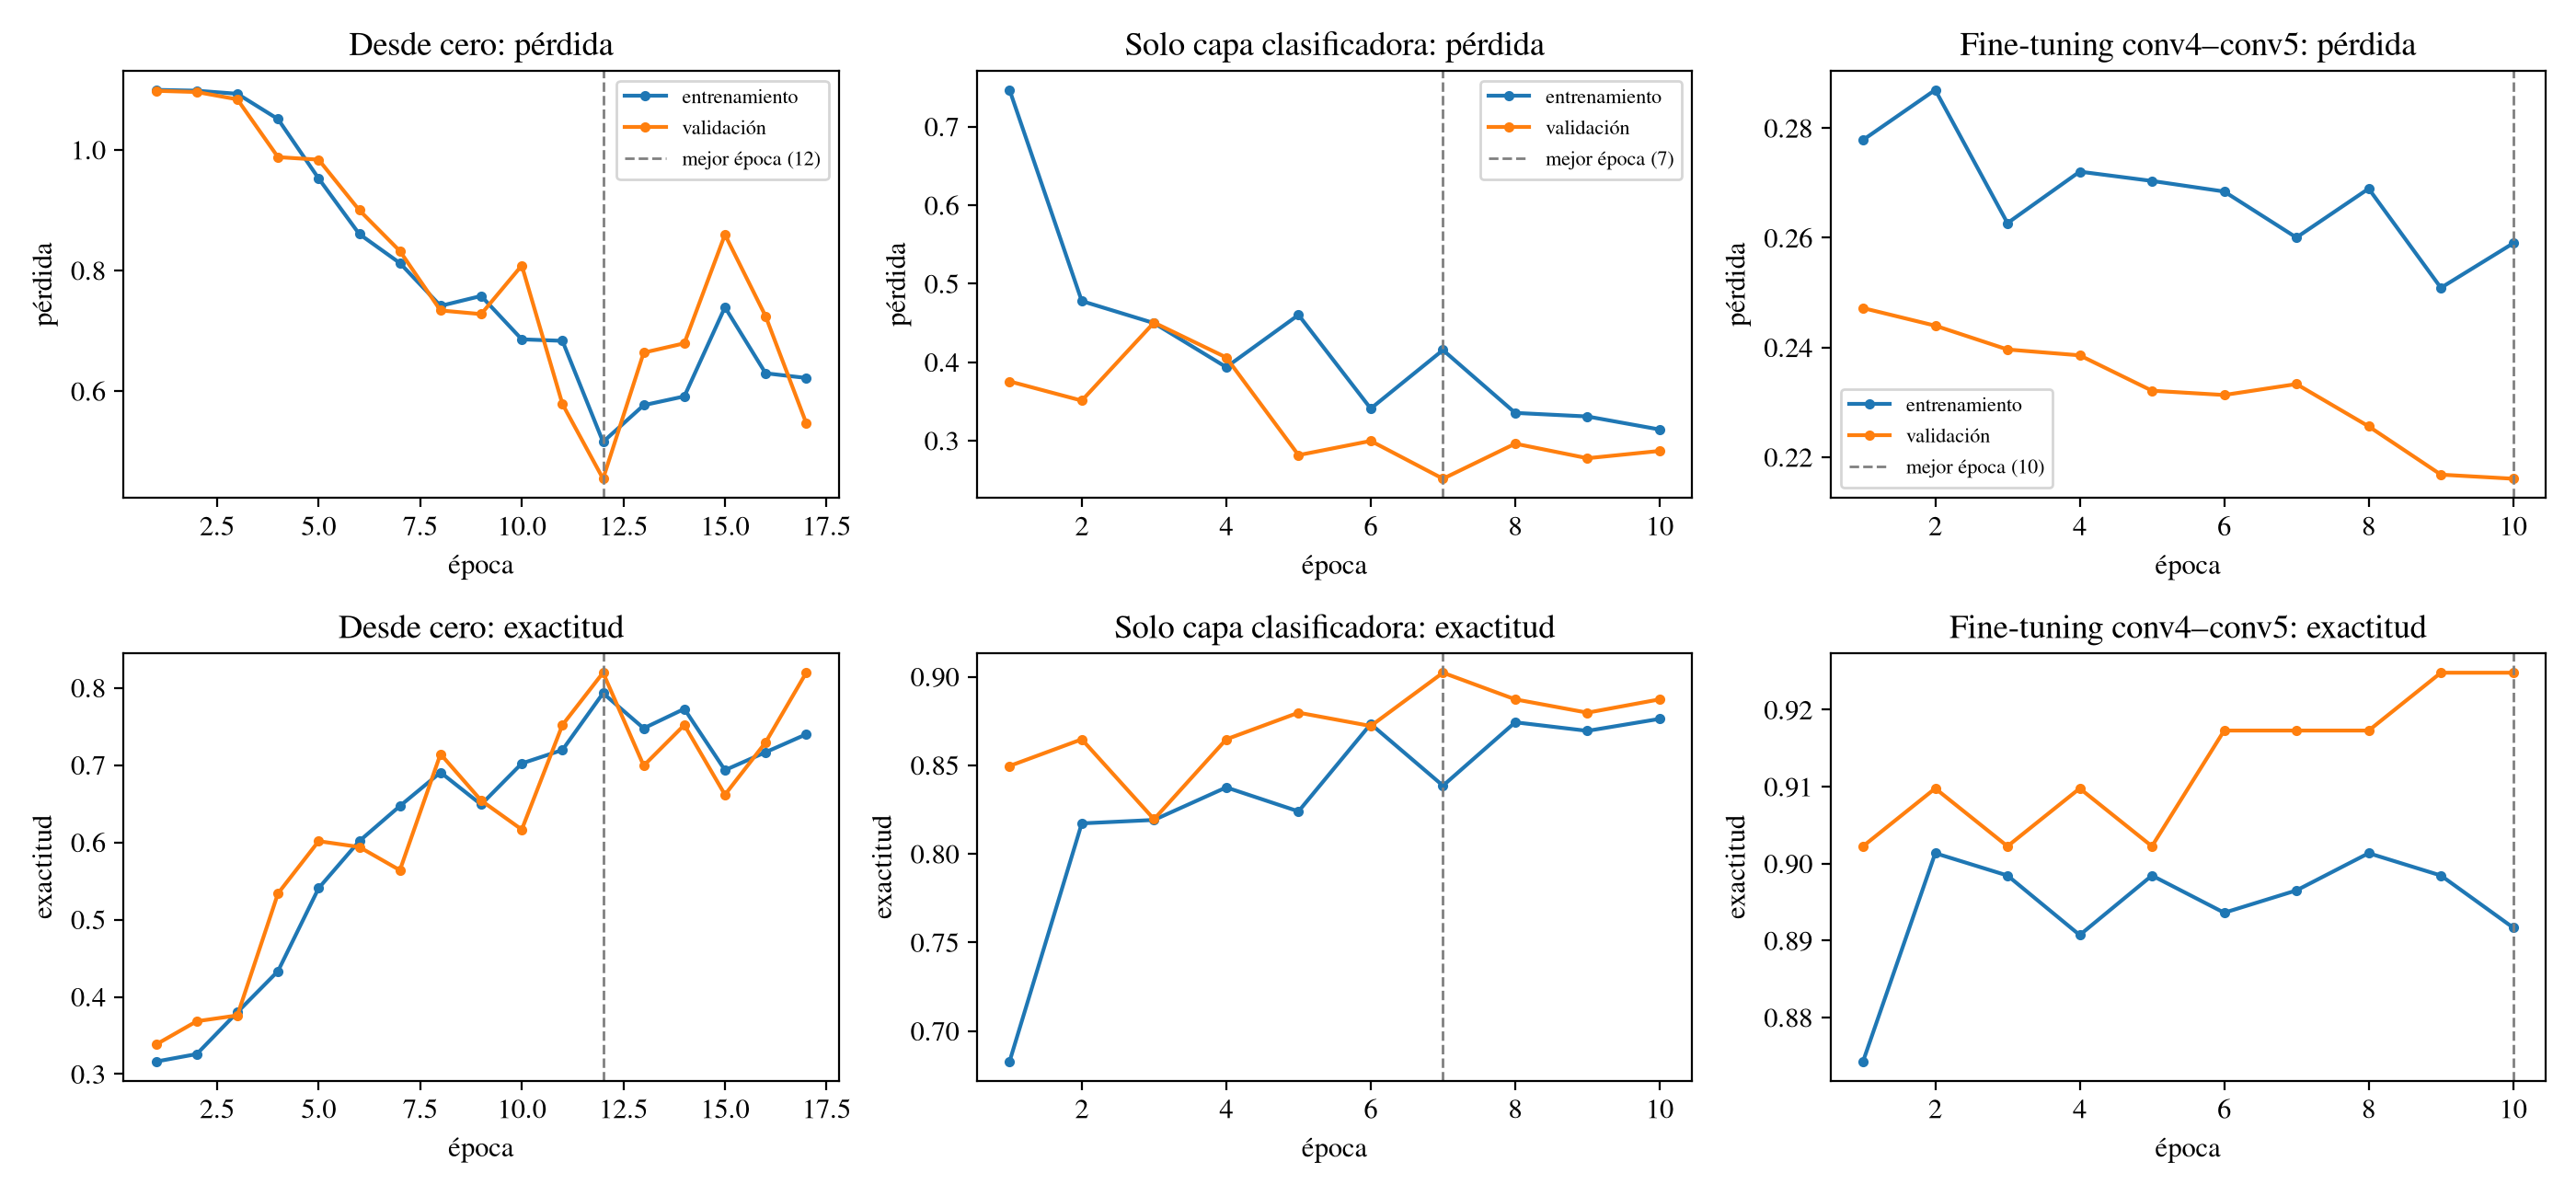
\includegraphics[width=\textwidth]{figures/curvas.png}
\nota{Entrenamiento y validación por época. La línea punteada marca la mejor época, cuyos pesos se
conservan.}
\end{figure}

\begin{figure}[!tbp]
\caption{Matrices de confusión en el conjunto de prueba}
\label{fig:matrices}
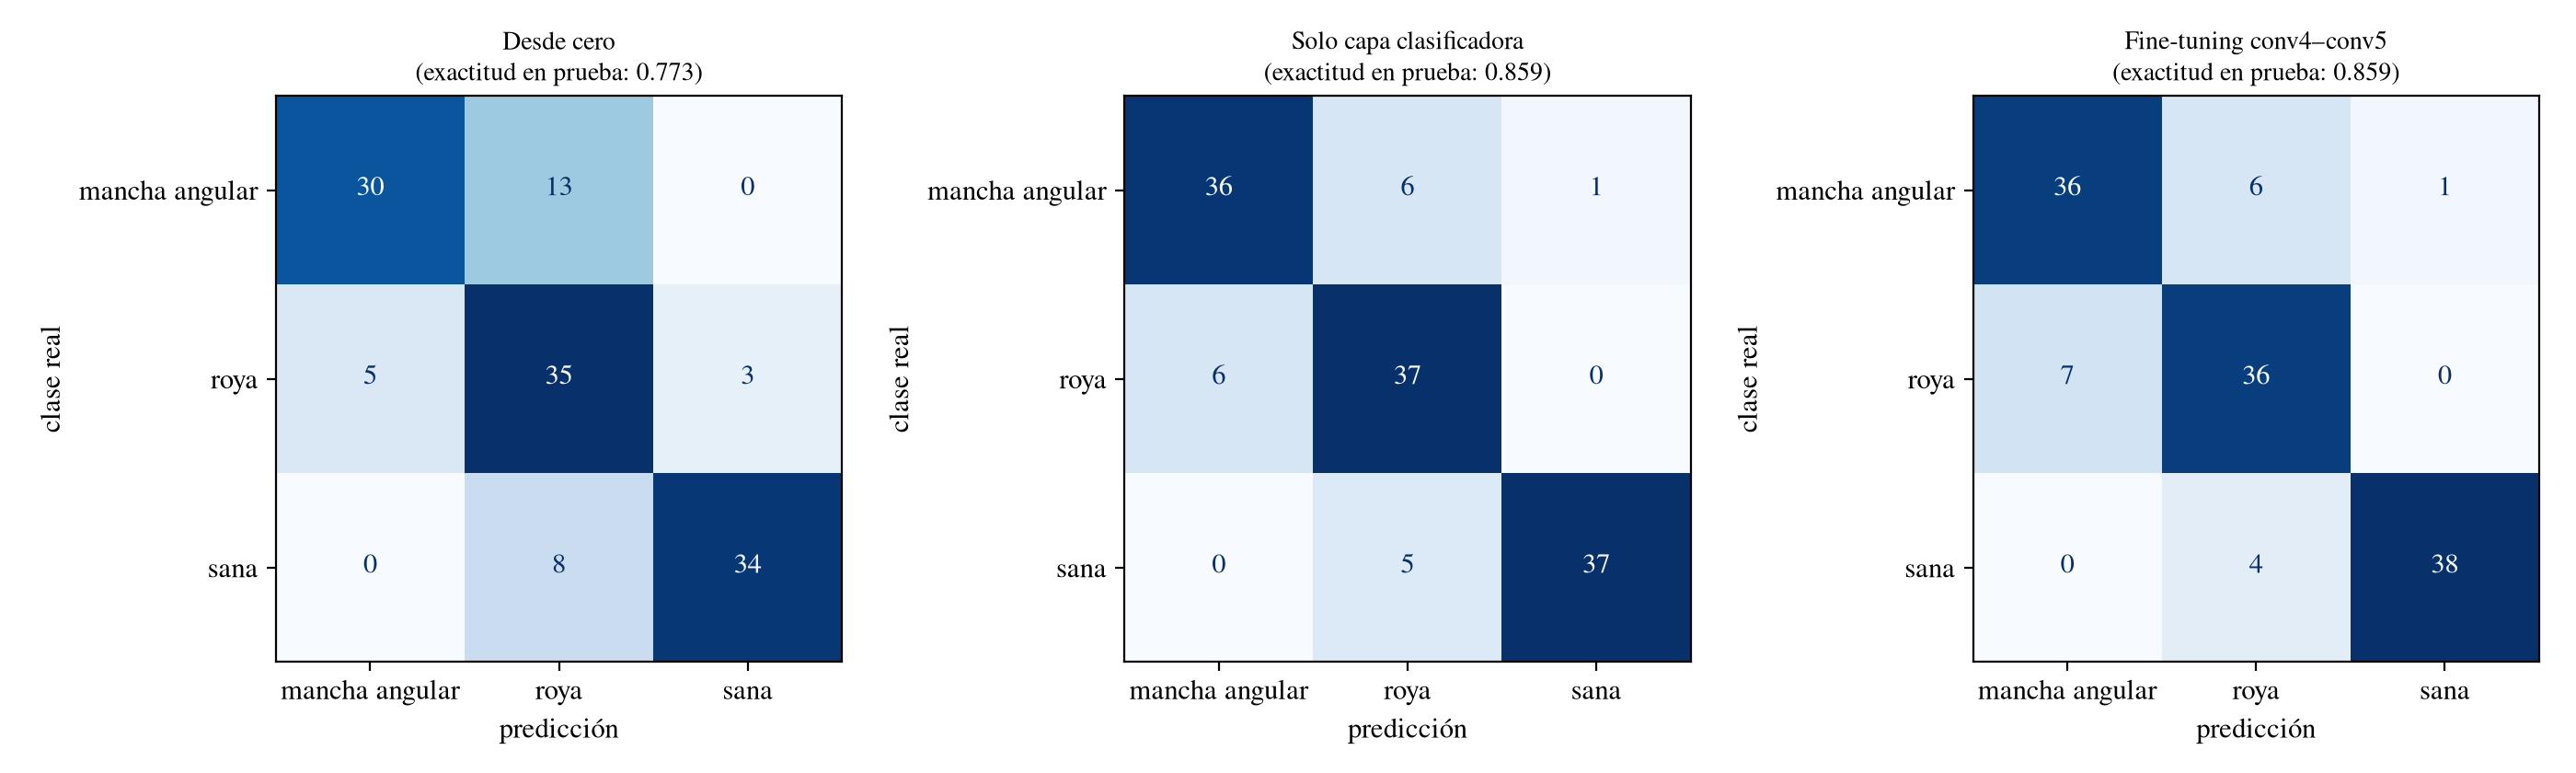
\includegraphics[width=\textwidth]{figures/matrices_confusion.png}
\nota{128 imágenes de prueba. Filas: clase real; columnas: predicción.}
\end{figure}

% ───────────────────────── 4. Conclusiones ─────────────────────────
\section{Conclusiones}

\begin{itemize}
  \item AlexNet tiene 3 bloques convolucionales con 5 convoluciones y 3 capas densas; el 96\,\% de sus
  61.1\,M de parámetros está en el clasificador. Usa ReLU y no fija optimizador.
  \item Permite agregar o reemplazar capas, congelarlas por separado y adaptarse a un problema
  específico, como demuestran las demos 2 y 3.
  \item La transferencia supera al entrenamiento desde cero (85.9\,\% frente a 77.3\,\% en prueba)
  entrenando 4600 veces menos parámetros y en mucho menos tiempo.
  \item El beneficio depende del problema: con imágenes sintéticas fáciles, el modelo desde cero fue
  suficiente; con fotografías reales y pocos datos, los pesos de ImageNet marcan la diferencia.
\end{itemize}

\printbibliography

\end{document}
